\section{Experiments}
\label{sec:experiments}

\subsection{Data Sets}


We use 5 \href{http://archive.ics.uci.edu/ml/datasets.html}{UCI classification
datasets}:, described as follows:

\begin{tabular}{| c | c |  c |}
\hline
Dataset & \# instances & \# features \\
\hline
Farms Ads dataset & 4,143 & 54,877 \\
\hline
Amazon Commerce reviews dataset & 1,500 & 10,000 \\
\hline
p53 Mutants dataset & 16,772 & 5,409 \\
\hline
Human Activity Recognition using Smartphones dataset & 10,299 & 561\\
\hline
URL Reputation dataset\footnotemark[1] & 2,396,130 (16000) & 3,231,961 (74113) \\
\hline
\end{tabular}

\footnotetext[1]{The dataset is too large so we used only one day of data out of totally 121 days in the dataset. See number in parentheses for specifications.}

\subsection{Results}

\subsubsection{MCMC based estimation}
Our MCMC sampling strategy that we described in section~\ref{sec:MCMCmethod}
converges. Figure~\ref{fig:MCMCconverge} is a plot of the iterations of the Markov 
chain for estimation on a subset of Farms Ads dataset. This is for MLE
estimation without any priors. We also 

\begin{figure}![htb]
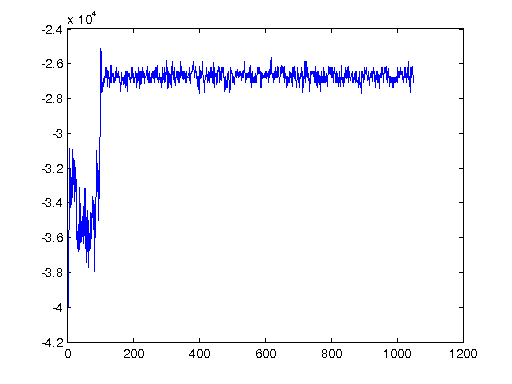
\includegraphics[width=1\textwidth]{samplingConvergence.png}
\caption{Markov chain convergence on Farms ads data. We take a sub-sample of
the dataset: 2000 rows and 100 columns}
\label{fig:MCMCconverge}
\end{figure}
